%%%%%%%%%%%%%%%%%%%%%%%%%%%%%%%%%%%%%%%%
% Chapter 3: Data synthesis
%%%%%%%%%%%%%%%%%%%%%%%%%%%%%%%%%%%%%%%%


Synthetic data generation is an iterative process that can be divided into three phases: the preparation phase, the data generation phase and the data evaluation phase. 

\vspace{10pt}
\begin{figure}[h!]
    \centering
    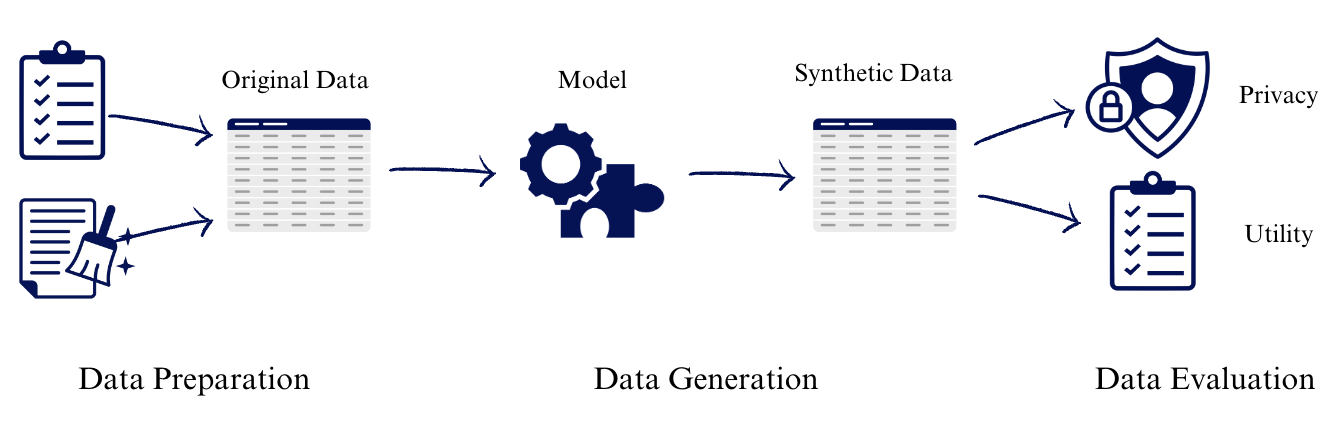
\includegraphics[width=\textwidth]{Images/Screenshot 2024-08-06 at 12.00.18.png}
    \caption{The Synthesis Process.}
    \label{fig:synthesis_1}
\end{figure}
\vspace{10pt}

\section{The data preparation phase}

The goal of the preparation phase is to determine the ideal characteristics of the synthetic data and to choose a fitting generation method.

\textbf{Step 1a: When creating synthetic data from scratch: determine the structure and characteristics of the synthetic data} \\
Generating synthetic data from scratch requires meticulous preparation to ensure that the artificial data accurately reflects the intended use case and properties. The preparation phase involves several key steps. When developing synthetic data based on domain knowledge, deep comprehension of the domain is crucial. This includes understanding the key variables, their relationships, and the underlying processes governing the real-world data. For example, generating a synthetic database of a population of prisoners requires knowledge about the characteristics of prisoners. Equally, when the goal is to generate synthetic legal text, knowledge of legal jargon is a requirement. Another key step lies in defining the objectives for generating synthetic data. Will the data be used for testing algorithms, simulating specific scenarios, or conducting replication studies (to name just a few examples)? Depending on the answer to this question, the key features of the synthetic data need to be identified, such as their specific statistical properties: distributions, means, variances, correlations, and other relevant statistical metrics. For textual data, the desired length, complexity, tone or linguistic patterns need to be determined \cite{el2020practical,soltana2017synthetic}. In a way, this process of generating synthetic data closely resembles the data generation process for real-world data. Thus, mimicking that generation process as closely as possible will ensure realistic synthetic data.

\textbf{Step 1b: When generating synthetic data to mimic real-world data: prepare the original dataset} \\
When generating synthetic data based on real-world data, it is still necessary to understand the key features of that data, such as distributions and relationships among variables for structured data, or patterns in language, sentiments, topic and structure for unstructured data, such as texts or audio. This knowledge is later required to evaluate the quality and usefulness of the synthetic dataset. In addition, data cleaning and preprocessing are crucial at this stage to ensure the quality and consistency of the real-world data, which serves as a benchmark for the synthetic data. Any mistakes, biases, outliers, special characteristics or irrelevant information need to be resolved or at least identified before the synthesis, as the synthesis process would mimic those mistakes. Finally, any additional requirements for the synthetic data, such as logical rules, need to be determined. For example, if the original dataset contains a variable classifying individuals as either adult or minor, as well as a variable on the specific age of the individual, the model may recognise that individuals classified as minor have a significantly lower age than those classified as adults, but it may be necessary to create a rule that the specific age of minors in the synthetic dataset must not exceed 17. \\

\textbf{Step 2: Choosing the right generation method} \\
There are several methods to generate structured and unstructured synthetic data, and the choice depends on the type and complexity of the data, as well as the specific requirements of the project. Some of these methods may require advanced statistical knowledge, whilst others are more accessible to researchers without advanced expertise in statistics or data science. Some general categories of these methods are presented here.
 
\textbf{Rule based methods} for synthetic data generation rely on predefined rules, algorithms or simulations that mimic the behaviour and interactions found in real-world systems. These methods are particularly effective when no prior data is available, but domain knowledge is well-understood and can be explicitly encoded into the data generation process. In some disciplines, there may already be mathematical models that can be used for simulations, such as epidemiological models on the spread of diseases that can be used as a guidance for the synthetic data \cite{ajelli2018rapidd,gonzales2023synthetic}. Rule-based models are also suitable for demographic simulations, if demographic rules and census data offer enough information to create an artificial population. Through sophisticated approaches such as Agent-Based Modelling, even complex interactions between individuals and macro-level dynamics can be simulated in synthetic data \cite{grinberger2017dynamic}. On the one hand, rule-based models can be highly tailored to specific domains, ensuring that synthetic data closely mimics real-world scenarios. Another benefit is that the rules through which the synthetic data is created need to be specified, which makes the data generation process transparent and understandable. On the other hand, it can be complex and time-consuming to create rule sets that accurately capture dynamic real-world behaviours. Additionally, synthetic data from rule-based methods can only include patterns and relationships which are known beforehand, thereby possibly excluding unknown but vital information. 

\textbf{Statistical models} use mathematical formulas to replicate the characteristics and relationships found in real data. For example, through random sampling, a model can generate synthetic data points from probability distributions that closely match the distributions observed in the real data. Thus, if the original data follows a normal distribution, synthetic data can be generated by sampling from a normal distribution with a similar mean and standard deviation as the original data. Other statistical models, such as copulas, may be more suited if one aims to model the dependency structure between multiple variables \cite{kamthe2021copula}. The vast variety of statistical models allows for flexible adaptation to different types of data and purposes for generating synthetic data. However, depending on the complexity of the original data, sophisticated statistical techniques and skills may be required to generate useful synthetic data. In addition, synthetic data generated through statistical models require a thorough validation to ensure that it accurately represent the real-world data \cite{pezoulas2024synthetic}. Also, statistical models often rely on strong assumptions regarding which distribution the data follows. These assumptions may not always hold true in practice. 

\textbf{Machine/Deep learning models} are used for generating more complex and realistic synthetic data. One example of a machine learning model are Generative Adversarial Networks (GANs). GANs involve two neural networks; one that generates synthetic data and one that evaluates it. They "compete" against each other, thereby improving the quality of the synthetic data over time \cite{wang2017generative}. Another example are Variational Autoencoders (VAEs), that learn to generate data by encoding the original data to grasp its key features and decoding these features into synthetic data points \cite{doersch2016tutorial,wan2017variational}. Bayesian networks require a map about the relationships between variables in the original data beforehand (e.g. based on expert knowledge), based on which they can learn about the probability that certain combination of features in the original data co-occur. This knowledge is then transferred into a synthetic dataset. These methods are powerful for creating high-fidelity synthetic data, but they require substantial computational resources and expertise and are thus not beginner-friendly. For textual data, language models such as GPT-4 are designed to generate and understand human language, such as grammar, syntax and semantics and replicate next text by predicting the next word or sequence of words \cite{li2023synthetic}. The benefit of machine learning models is their flexibility to learn and replicate complex patterns in data without heavily relying on assumptions, next to their ability to quickly scale to large datasets. However, compared to statistical and rule-based models, machine learning models are much more likely to replicate sensitive information in the synthetic data, due to over-fitting. In other words, these models may replicate the original data \textit{too} well. In addition, training these models can require (large amounts of) training data that the researchers needs to have available in addition to the data that needs to be replicated. Also, training and fine-tuning these machine models can require more advanced knowledge of computations.


%%%%%%%%%%%%%%%%%%%%%%%%%%%%%%%%%%%%%%%%

\section{The data generation phase}


\textbf{Step 3: Synthetic data generation} \\
The actual synthesis process is heavily dependent on the chosen model and the type of data that need to be synthesised. In general though, each of these models studies the real data or rules through which new synthetic data needs to be developed to determine the various patterns, relationships, and statistical properties within the original data or rules. 
Once the model has satisfactorily learned the properties of the real data, it can be utilized to generate new data points. This new data is not copied directly from the real data but is generated based on the patterns the model has learned, or rules that have been fed to the model. 

%%%%%%%%%%%%%%%%%%%%%%%%%%%%%%%%%%%%%%%%

\section{The data evaluation phase}

\textbf{Step 4: Evaluation of synthetic data} \\
Evaluation is a critical step in the process of generating synthetic data. When synthetic data is created from scratch, theory or domain knowledge, it needs to be evaluated against the rules and requirements set out at the beginning of the process. When synthetic data is generated to mimic real-world data, it needs to be evaluated on its similarity to the original data. When synthetic data is generated to ensure privacy, it needs to be evaluated and checked using controls for privacy. More detailed explanation on the evaluation of synthetic data is described in the following chapter. When the outcome of these evaluations does not align with the requirements for the synthetic data, the process of synthesising data needs to be repeated and adapted where necessary. As such, the synthesis of data becomes an iterative process.


\textbf{Optional: Further data anonymisation} \\
To ensure privacy, further steps may be taken to verify that the synthetic data does not contain any identifiable information. Even though synthetic data is inherently safeguarding personal information by generating artificial datapoints that do not relate to real-world persons, additional precautions can be implemented to safeguard against potential privacy risks, such as leaving out variables with highly sensitive information or by adding differential privacy measures after the synthesis. 


%%%%%%%%%%%%%%%%%%%%%%%%%%%%%%%%%%%%%%%%


\section{Open-source tools for synthetic data generation}

Synthetic data is not a new invention. Several open-source tools already exist that make the generation of synthetic data easier, due to their accessibility, flexibility, and the supportive communities that often accompany them. A few note-worthy open-source options are presented here, with a more comprehensive list in the appendix.

\textbf{Synthetic Data Vault} \\
The Synthetic Data Vault (SDV) is a comprehensive library that offers a variety of methods for generating synthetic data \cite{patki2016synthetic}. It supports generating tabular, sequential, and relational data. SDV utilises machine learning models to capture the distributions and relationships in the original data, ensuring realistic synthetic data generation. It is particularly useful for data scientists who need a robust, all-encompassing tool for different types of data. Next to synthetic data generation, it also incorporates various metrics for evaluating synthetic data quality. \textbf{Ease of use}: Moderate. SDV offers comprehensive documentation and examples, but understanding its full capabilities may require more extensive data science knowledge. \textbf{Programming language}: Python. 

\textbf{SynthCity} \\
SynthCity is a comprehensive library for synthetic data generation and evaluation \cite{qian2024synthcity}. It includes a wide variety of models for synthetic data generation, ranging from more classical machine learning algorithms, to Bayesian Networks, to advanced algorithms like GANs and VAEs. It includes methods for both tabular and imaging data generation. Furthermore, it contains a wide variety of metrics for comprehensive evaluation of synthetic data quality. \textbf{Ease of use}: Moderate. As in the SDV, SynthCity offers direct plug-and-play capabilities, but understanding its full potential may require more extensive data science knowledge. \textbf{Programming language}: Python. 

\textbf{YData} \\
YData Synthetic is an open-source tool that provides a user-friendly interface for generating synthetic data \cite{ydata}. It leverages GANs to create realistic data, focusing on enhancing the quality and diversity of synthetic datasets. \textbf{Ease of use}: YData Synthetic is designed to be easy to use, with straightforward interfaces and tutorials that make it accessible even for those with limited data science expertise. \textbf{Programming Language}: Python.

\textbf{Faker}\\
Faker is a lightweight library that generates fake data for various uses, including testing and development \cite{faker}. It can produce names, addresses, text, and other common data types. While not as advances as other tools for complex datasets, Faker is highly useful for quickly generating simple, structured synthetic data. \textbf{Ease of use}: High. Faker is extremely easy to use, with simple commands to generate various types of fake data quickly. \textbf{Programming Language}: Python. 

\textbf{Synthpop} \\
Synthpop is an R package focused on generating synthetic versions of data sets for statistical disclosure control \cite{nowok2016synthpop}. It is particularly popular in social science research, where it helps in creating synthetic datasets that preserve the statistical properties of the original data while protecting privacy. It relies on decision trees to sequentially populate synthetic features, to ultimately generate a synthetic dataset. \textbf{Ease of use}: Moderate. Synthpop provides extensive documentation, but some familiarity with statistical concepts and R programming is necessary. \textbf{Programming Language}: R (Python wrapper also available). 
